\documentclass{beamer}%
\usepackage[T1]{fontenc}%
\usepackage[utf8]{inputenc}%
\usepackage{lmodern}%
\usepackage{textcomp}%
\usepackage{lastpage}%
\usepackage{graphicx}%
%
\title{Yair company}%
\author{Your Name}%
\date{\today}%
%
\begin{document}%
\normalsize%
\maketitle%
\section{Introduction}%
\label{sec:Introduction}%
\begin{frame}%
\frametitle{Introduction}%
This slide introduces the company and provides context.%
\end{frame}

%
\section{Data}%
\label{sec:Data}%
\begin{frame}%
\frametitle{Data}%
This slide contains the data used in the analysis.%
\begin{itemize}%
\item Hey%
\item $2^4 = ?$%
\end{itemize}%
\end{frame}

%
\section{Analysis}%
\label{sec:Analysis}%
\begin{frame}%
\frametitle{Analysis}%
This slide presents the analysis of the data.%
\end{frame}

%
\section{Classifications}%
\label{sec:Classifications}%
\begin{frame}%
\frametitle{Classifications}%
This slide presents the classifications based on the analysis.%
\end{frame}

%
\section{Visualizations}%
\label{sec:Visualizations}%
\begin{frame}%
\frametitle{Visualizations}%
This slide contains a simple line graph.%


\begin{figure}[h!]%
\centering%
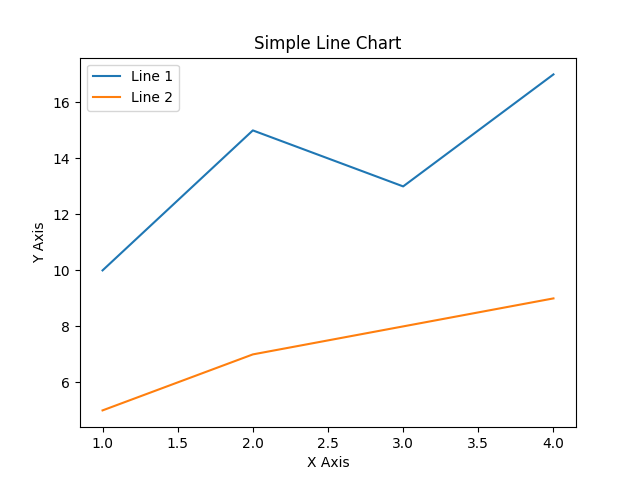
\includegraphics[width=80mm]{line_chart.png}%
\end{figure}

%
\end{frame}

%
\section{Anomalies}%
\label{sec:Anomalies}%
\begin{frame}%
\frametitle{Anomalies}%
This slide presents the detected anomalies in the data.%
\end{frame}

%
\section{Prediction}%
\label{sec:Prediction}%
\begin{frame}%
\frametitle{Prediction}%
This slide presents predictions based on the data.%
\end{frame}

%
\section{Conclusions}%
\label{sec:Conclusions}%
\begin{frame}%
\frametitle{Conclusions}%
This slide summarizes the key takeaways from the analysis.%
\end{frame}

%
\end{document}